\documentclass[USenglish,oneside,twocolumn]{article}

\usepackage[utf8]{inputenc}%(only for the pdftex engine)
%\RequirePackage[no-math]{fontspec}%(only for the luatex or the xetex engine)

% Do not change the template unless necessary
% Changing font sizes, margins or similar to make your project report appear longer
% than it is will lead to a failed exam.
\usepackage[big]{dgruyter_NEW}

\usepackage{graphicx}


\usepackage[backend=biber,natbib=false]{biblatex}
\addbibresource{references.bib}

% You can remove this include
\usepackage{blindtext}
  
\begin{document}
	% Do not enter real names for the blind review.
	\author*[1]{Corresponding Author}
	\author[2]{Second Author}
	\author[3]{Third Author}
	\author[4]{Fourth Author}
	
	% Do not enter your real email address for the blind review.
	

	\title{\huge Post Quantum Key Exchange Mechanisms for the IOT}

	\runningtitle{Running title}

	\journalname{Internet of Things Projects}
	\startpage{1}
	
 	\begin{abstract}
		{Innovations such as post-quantum cryptography have created new needs for secure connections between devices that will be part of a long-term ecosystem. Currently, all existing Internet of Things (IoT) devices use asymmetric key based cryptography, enabling an advanced level of security today but may possibly be compromised by quantum computers in the future. Therefore, all current secure communication channels with IoT devices will ultimately end with an encrypted and decrypted view of the data ever exchanged through them. The implementation and use of quantum resilient security in very small form-factor IoT devices are still being addressed because of the limitations imposed on these small embedded electronic devices, in terms of available RAM/memory, energy/battery life, bandwidth, etc. A post-quantum key agreement protocol for the IoT will be developed in this project to fill a continuing gap in this area. A pair of IoT devices (PineCone/BL602) will demonstrate a proof-of-concept by communicating across a local Wi-Fi network using CoAP as the application layer protocol. First, a post-quantum key establishment mechanism (KEM) from the Kyber family, designated as ML-KEM by NIST will establish a shared secret between the two nodes. This shared secret will subsequently be used in tandem with an encryption/authentication mechanism based on AES-CMM, providing confidentiality and integrity during CoAP communications.Instead of creating a variety of cryptographic primitives, the focus of the current project is to facilitate integration and to develop a user-friendly experience.Wi-Fi/IP setup, CoAP communication, key establishment and AEAD encryption/authentication are all separated by implementation to make the protocol logic modular.. The long-term post-quantum key pair will be maintained in the internal flash memory of the gateway node, while the sender will engage in the encapsulation of the secret key via a straight CoAP handshake over a secure channel, thus creating a session key. Thereafter, the messages are AEAD encapsulated with key nonce management. Also the states transitions from handshake to secure data.
        In order to verify that our protocol is functioning we also examined the traffic patterns using typical network analysis tools, e.g. Wireshark.In conclusion, this project provides a repeatable design methodology for developing a Quantum Resistant Key between a small CoAP-based device and an arbitrary other system. The project has involved a theoretical migration from a Concept design, then development of a Demonstration Prototype, then a Complete End-to-End Demonstration on a commercial IoT Board. This set of components can also be leveraged for other similar platforms. }
	\end{abstract}
	\maketitle

	\section{Introduction}
    The internet of things, nowadays, has grown into a dense IOT device network that can  sense,process and share physical world information. However, one of the challenges involved in this dense IoT Device Network is that with the rising number of IoT devices, there has been a scene where their data has been left insecure due to their use of Public Key Cryptosystems like RSA which are suceptible to Quantum Computer attacks. Indeed, it is important to note that "Harvest Now – Decrypt Later" has become a reality for those that seek to exploit this data when Quantum Computing technology becomes available. There has, therefore, been a rising challenge for various types of IoT devices that will be used for a long period of time and are also difficult to upgrade.
    Our IoT system that is secure from the threat of quantum computing takes care of this issue by providing a method for establishing keys post-quantum in actual IoT applications where it can be used safely every day. We do this through a very specific way we have designed the IoT architecture that will utilize PineCone BL602 cores to form nodes; these nodes will communicate using Wi-Fi, and the application data will be exchanged using CoAP, which is very low overhead UDP based way of transferring data as opposed to standard HTTP. In addition to using the normal method of key exchange, we provide a method of establishing a post-quantum key using our novel key encapsulation mechanism from the ML-KEM/Kyber Family; this allows for the creation of a new secret key between a sender node and a gateway node that will then be used to establish a shared symmetric session key; this key will be utilized by the sender node and the gateway node to offer all CoAP payloads legitimate security through AES CMM Based Authenticated Encryption when the CoAP path is considered trusted and trusted over secure means.
    The design principle of this system is based around a clean, modular architecture. This implies that the architecture maintains clear, seperable boundaries between the transport layer, post-quantum key establishment and data security functions, so that each of those components may be operated and exchanged independently. CoAP provides the request/response model making use of application messages, the post-quantum KEM provides the initial session key setup and AES CMM Authenticated Encryption offers a secure transport of data. The keys and nonces are handled during the associated transitions between the handshake and data transmission steps with secure cryptographic parameters. Along with "making it work," the goal of this project is to evaluate whether it can actually be implemented on a limited hardware platform. When profiled using the PineCone boards, it has assessed the code size, RAM utilization, and the functionality used for the initial connection setup to establish the communication protocol between devices and during the subsequent regular communications of messages. In order to make it easier to understand information regarding the communication patterns between these devices, a separate communication-sniffing configuration has been created to capture all communications occurring over-the-air. This communication has then been analyzed using tools such as Wireshark, which has been used to visualise the communication in a very granular way
    
    This paper provides the clearest and most inclusive outline of a design for a full, end-to end, postquantum secure IoT system incorporating every aspect of a standard/standardised cryptography components of postquantum IoT systems to ensure that IoT systems will meet the requirements of complying with postquantum security standards (or standardised). In addition, this paper discusses the particular requirements for secure communications essential to IoT systems. To illustrate the path to designing such an IoT System, this report provides a high-level overview of several types of public-key cryptography methods that are vulnerable to Quantum Computing attacks, describes how Constrained IoT Nodes and CoAP-Based Designs (Client/Server) are affected by this vulnerability, describes the Prototype Hardware and Software Designs and Communication Mechanism used to create the prototype's proof-of-concept implementation(s), describes how ML-KEM/Kyber and AES-Based AE were used to enable CoAP-based messaging for secure communications in the prototype, and finally discusses the results of testing the prototype implementations and their associated traces to provide an understanding of the feasibility of integrating Quantum Security support with small IoT devices and any possible trade-offs involved in expanding Quantum Security support to these devices.
	\label{sec:intro}
	
	\section{Background}
    ML-KEM, the respective key encapsulation mechanism, is specified in a NIST Federal Information Processing Standard as a publicly-key based lattice-based scheme with a security reliance on the hardness of the Module-Learning with Errors problem (MLWE problem), which basically challenges an attacker to find hidden structure in a set of noisy linear equations, a problem that is assumed to be unhackable by either classical or quantum computers ~\cite{Naya2025}. It is specified in three different instances: ML-KEM-512, ML-KEM-768, and ML-KEM-1024, with increased sizes but also increased securities. The ML-KEM instance that is used within this project on the pinecone BL602 microcontroller is ML-KEM-512, which is essentially the smallest of the ML-KEM instances, providing a similar level of protection for a 128-bit symmetric-key block cipher, though still being reasonable enough in terms of computational power for use within embedded systems, our focus device is pinecone bl602~\cite{Naya2025}.The ciphertext size is 768, the secret shared size is 32, the size of the public key is 800 and the matching size is 1632..~\cite{Naya2025}
    
    The ML-KEM, a key encapsulation mechanism, is based on the CRYSTALS-Kyber algorithms that was selected as the preferred key encapsulation mechanism in NIST's post-quantum cryptography standardization process. In the last few years, as the CRYSTALS-Kyber family of algorithms matured, many more research papers have been published investigating how to best implement CRYSTALS-Kyber in microcontroller environments and for devices powered by limited battery power (e.g., Internet of Things processors). In particular, implementation of CRYSTALS-Kyber on an BL602 Pinecone microcontroller as described above indicates that it is feasible to take advantage of post-quantum (PQ) key-exchange mechanisms within interactive systems running on microcontroller platforms, and that some tasks may be completed in a matter of milliseconds by executing on two cores. ~\cite{al2025}
    
    Our scheme takes the common design of long-term server key, ephemeral client encapsulation, which is typically recommended when constructing KEMs when used as part of key-establishment primitives. The Gateway party holds a key of ML-KEM-512, which will not be changed, and the Sender one gets the matching part of the key, encapsulation is carried out among this part and the public one. It produces a common shared 32-byte secret, which is communicated only with the two parties, and which is as hard as MLWE. To apply it as an encryption key, instead of direct application, the secret is computed through HKDF-SHA-256, to generate a 128-bit AES-CCM encryption key, specifically designed to suit the task in the application, based on a key derivation mechanism, which fits in the KEM + KDF + AEAD construction, which is recommended to mix such primitives in the NIST guidelines, as cited in. ~\cite{Naya2025}

    On the protocol domain, the solution uses the Constrained Application Protocol (CoAP), a web transfer protocol specifically designed for constrained nodes, which is characteristic of IoT scenarios ~\cite{shelby2014}. CoAP is similar to HTTP in that it supports the REST paradigm, with GET, PUT, and POST requests on URIs, but packages it all in a binaryrepresentation on top of UDP, as opposed to TCP. It supports confirmable messages with a lightweight acknowledgment mechanism, which is useful when messages might be lost, but is also available in a non-confirmable message when low latency is desired. This is particularly useful when a microcontroller wants to support web interactions. ~\cite{shelby2014}

    To formally state the cryptographic protection of such application data, the CBOR Object Signing and Encryption (COSE) specification applies a set of conventions to the compact binary serialization of CBOR to provide a standardized way to encode keys, signatures, message authentication codes, and encrypted data ~\cite{schaad2022}. The COSE specification establishes conventions for algorithm identification as well as conventions for handling application-specific, but still authenticated encryption schemes, such as AES-CCM with varying tag lengths, which are currently included in the COSE registry. AES-CCM is a counter-mode with aCBC-MAC encryption scheme, which provides integrity as well as confidentiality with a single call, which is especially used in low-rate wireless Personal Area Networks, such as IEEE 802.15.4 and ZigBee, for securing short messages when minimizing CPU resources, as in IoT scenarios ~\cite{Naveen2024}.

    The prototype that is developed as a part of this project is based on CoAP and COSE, but is not dependent on the full implementation of COSE/CBOR, as a choice is made to keep the code size small to match RAM requirement of Pinecone. The REST API is offered on application data with CoAP on top, with an AES-CCM layer in the stack beneath it, which is roughly on the same level as CoSE, with regard to choice of algorithms and generation of keys. The ML-KEM establishes a common secret with the Sender as well as the Gateway, HKDF is a single 128-bit AES-CCM key, which is used to encrypt the payload of CoAP messages, as well as the contextual detail, which is implicitly bound to a CoAP transaction, but is not conveyed within a COSE message ~\cite{shelby2014} ~\cite{schaad2022}.

    Generally, the research is an extension of the existing literature on the subject of resource constrained post quantum cryptography which is now being performed on a microcontroller based IoT nodes ~\cite{Tao2024} ~\cite{asif2021} ~\cite{al2025}. The already existed literature reviews on the subject compare the performance of different solutions on the basis of execution time, RAM requirement, size of code, and energy cost of energy. It is generally agreed that post quantum solutions are more expensive than the currently deployed elliptic curve solutions, but it is possible to manage them with relatively lightweight IoT systems with a considered eye of cost limitations Specifically, key exchange, implemented using KEMs is manageable even when the key exchange is conducted to be set up, yet with minimal impact in total cost of energy. Conversely, these contributions highlight the necessity to think in terms of cryptographic design in general on migration to PQC, and not just to apply isolated primitives. Within the IoT protocol space, a variety of proposals have been suggested which attempt to serve the end-to-end protection within the limitations of the devices themselves. One of these is Object Security for Constrained RESTful Environments (OSCORE), which is a prominent solution based on CoAP and COSE to provide application-layer payload security between parties, independent of which mechanism of transportation is employed ~\cite{sel2019}. The OSCORE demonstrates that the protection of encryption and integrity can be offered on the level of objects and the presence of middleboxes like proxies that may still send the messages with the protection without paying attention to them. We are more or less the same design but in two important ways.On the one hand, our implementation substitutes classical Diffie-Hellman key agreement with ML-KEM-512, which provides the advantage of post-quantum protection on the design of the key agreement procedure. On the other, our design specifically optimizes for a minimal authenticated encryption channel, keeping in mind the very limited memory constraint of microcontrollers with a Wi-Fi connection. Related research on forensic-capable Wi-Fi access points and IoT traffic analysis frameworks has illustrated the use of low-cost hardware to timestamp and export traces of wireless activity for external analysis to facilitate debugging, observation, and incident response in embedded systems scenarios ~\cite{fabio2023} ~\cite{tina2021}. Such solutions identify the importance of having, in addition to secure communication mechanisms, knowledge of the generated traffic behavior. Having in mind this perspective, the prototype developed within the project represents a real-world approach to making IoT stacks post-quantum secure. It brings together a structured post-quantum secure KEM, conservative key derivation practice, combined with a clearly understood AES-CCM with CoAP application layer message semantics. On the other hand, the design takes into consideration a set of best practice learnings from the literature, which views the design goals of structure, observability, and implementation considerations as fundamental, thus filling a significant gap that exists within high-level post-quantum proposals and more implementation-oriented systems perspectives ~\cite{Tao2024} ~\cite{asif2021} ~\cite{sel2019} ~\cite{fabio2023} ~\cite{tina2021}
    
	\label{sec:background}
	
	
	\section{System Design and Implementation}
	

    \begin{figure}[t]
  \centering
  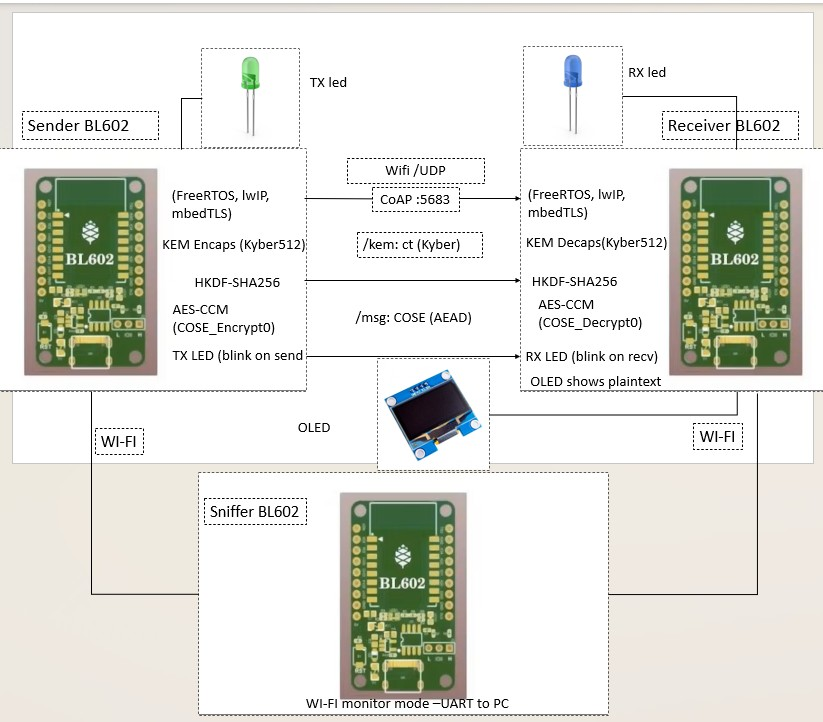
\includegraphics[width=\columnwidth]{IOT.jpg}
  \caption{System architecture.}
  \label{fig:bg-arch}
\end{figure}

    \subsection{Hardware Integration}
    The hardware of all three microcontroller boards is the same. All three are PineCone boards based on the Bouffalo Lab BL602 microcontroller. They are both USB powered and have a serial interface with a debug and logging interface on BL602. Development and testing is also easy: one can power the board with a laptop and use the same cable to read debug prints, timing measurements and error messages. One of the BL602 GPIO pins on the Sender and the Gateway is used to provide an external status LED. This LED is briefly lit up by the firmware after the key cryptography operations have completed successfully, such as after a key exchange, a successful decryption or a successful authentication tag verified correct. These brief spurts of feedback are highly immediate: although the serial console may not be open, a brief look at the boards can be used to tell the difference between a protocol being underway and the onset of a failure.The Gateway includes an additional peripheral: a small OLED display that is connected to the BL602 I2C pins of the microcontroller. Upon power-up, the Gateway firmware implements some simple functions that enable users to clear the display, position a text cursor and render ASCII characters using a bitmap font. If there is an active secure session and the user has successfully decrypted a previously encrypted message, the message content will now be presented on the small OLED screen. This means that messages displayed on the Gateway can only be read by the user when both post-quantum key establishment and authenticated encryption and decryption using an associated data (AEAD) scheme have been completed successfully.

    The Sniffer node is intentionally designed as a very minimal device.It uses pinecone device platform as well. To maintain the same USB power / serial debug architecture, all other displays, LEDs and lights are integrated directly onto the Sniffer. The Sniffer also operates in a monitor mode, which allows all frames that it detects on the given channel to be logged and subsequently packaged into a binary file containing time and length information. All captured frames are then immediately written to the USB serial port and subsequently transmitted to the host.This makes the Sniffer firmware lean and targeted at its one and only goal of making the microcontroller a low-cost, all-night wireless tap.

    \subsection{Software Development}
    Initially, the use of the BL602 microcontrollers enables firmware development for a limited firmware stack for each of the PineCone boards (the Sender board, Gateway board, and Sniffer board) that allows CoAP-over-UDP communication to be performed in a secure manner. Each of the three boards uses the C/C++ programming language and is developed with the use of the BL602 SDK. Each of the firmware applications runs on FreeRTOS (a small real-time operating system) and has a network stack named lwIP.

    The three PineCone boards all share a common start-up pattern based on FreeRTOS and the use of lwIP:

    \begin{enumerate}
    \item System Initialization:  each node when the reset occurs will execute its microcontroller core system initialisation such as clock and memory, uart, led gpio pins.
    \item Wi-Fi Connection: A Wi-Fi specific, process is charged with the responsibility of configuring the radio to act as a station, connect to the access point with pre-programmed credentials and wait to receive the response of DHCP, i.e., giving the node an IPv4 address. Once the node has received its IPv4 address, the Wi-Fi-specific task will print the networking information to the serial console and then set a global flag indicating that the node is now ready to communicate over the network.
    \item Application Start-up: Once the global flag indicating that the node is network-ready has been set by the Wi-Fi task, an application-specific task will wait until the global flag is set and then, when the flag is set, will begin executing the proper logic associated with the Sender board (Sender), Gateway board (Gateway) or Sniffer board (Sniffer).

    \end{enumerate}

    \subsection{Implementation}
    Once initialized, each PineCone (BL602) begins executing an application task depending on its specific role:
    \begin{enumerate}
    
    \item Pinecone(gateway):
    
    \begin{itemize}
    \item It holds a long term ML-KEM-512 keypair in flash memory and provides the Sender with the public key.
    \item Listens for CoAP requests on UDP.
    \item Decapsulates using ML-KEM, calculates the AEAD key with HKDF-SHA-256, then decrypts or verifies AES
    \item Anti-replay processing (message ID / nonce / sequence checking) is applied before accepting application data.
    \item Prints the decrypted message to the local OLED screen.
    \end{itemize}

    \item Pinecone(sender):

    \begin{itemize}
        \item It uses the Gateway public key for the ML-KEM-512 encapsulation procedure to derive the shared secret.

        \item Performs the HKDF-SHA-256 function to derive the 128-bit AES

        \item Creates a minimal CoAP over UDP message, then encrypts/authenticates the message using AES-CCM

        \item Rejects Duplicates/unexpected messages with freshness rules

    \end{itemize}

    \item Pinecone(sniffer)

    \begin{itemize}
        \item Runs in Wi-Fi monitor mode to capture IEEE 802.11 frames that are nearby.
        
        \item Streams the frames over UART/serial to a host-side decoding script

        \item This is then decoded for analysis in Wireshark to look for any anomalies in repetition rates characteristic of a replay attack. The Sniffer PineCone sends the captured 802.11 frame data to a host computer through the serial connection. A small decoding script on the host computer translates the captured data into a form that can be opened as a capture interface. This means that the data can then be captured and filtered in real-time using Wireshark while the application data is encrypted with AES-CCM. 
    \end{itemize}

    \end{enumerate}

    \section{Evaluation and Results}
    \subsection{Functional Behaviour}
    The system was consistent across the repeated runs. The reset made both Sender and Gateway the Wi-Fi network members, where they received IP addresses through DHCP and displayed them in the serial console. After the network was prepared the Sender sent a CoAP request to the public-key resource of the Gateway and received as always a response whose payload length corresponded to the ML-KEM-512 public key.With this key, the Sender then transmitted a second CoAP POST which took the ML-KEM ciphertext along with the AES-CCM encrypted payload. According to the logs of the Gateway, CoAP was correctly parsing, after which there was a successful decapsulation and decryption. The plaintext that was recovered was also displayed on the serial console and on the OLED display, thus verifying that the message content is only learned by the Gateway. LEDs on the Sender and Gateway would momentarily flash on every successful run. On the whole, these observations demonstrate that CoAP, ML-KEM, AES-CCM and persistent key storage are collaborative as a full-fledged end-to-end system.
    \subsection{Performance Measurements}
    Cryptography routines were embedded in a timer that had a timing resolution of milliseconds. The ML-KEM-512 decapsulation processing on the gateway had a time requirement of approximately 11 to 12ms (same as the time required for ML-KEM-512 encapsulation). Based on the measured values of the short status message used in the demonstration, the processing of AES-CCM Encryption and Decryption all completed under 1ms and effectively fell below the resolution of the timer; therefore, obviously, the post-quantum overhead is the primary factor in the timing. The latency timing values will be acceptable within the common latency budgets for IoT devices and applications. A single delay of several ten milliseconds for a one-time configuration of a session is marginal compared to typical network and application delay. The memory used was within the normal limit of the capabilities of the boards. The ciphertexts and keys are stored in static buffers, while the payload for CoAP security will be stored in easily accessible RAM. Because the application is non-dynamic, it will be considerably easier to estimate resource consumption in the worst-case scenario.
    \subsection{Packet level analysis}
    The Sniffer node captured traces which were then viewed in Wireshark and provided a network-level overview of the overall system. In the packet captures we see ARP and DHCP traffic as such traffic occurs when the board connects to the network. A subsequent CoAP POST message containing the public key was sent from the sender to the gateway, WS displays CoAP headers and the data itself as a block equal to the size of the public key. Subsequent data messages were sent using a different larger CoAP POST message, the payloads travelled as ML-KEM encrypted ciphertexts of 768 bytes in size along with AES-CCM nonce, the encrypted data and tag. CoAP has complete decoding capabilities for all of its header types and only the payload consists of random bytes created from proper application of encryption of the activity on the network. Synchronizing this with LED flashes and serial data, along with OLED information, will allow for correlation between what is being performed by the device and what you see on the wireless link

    \section{Conclusion and Future work}
    This project has introduced the design and implementation of post-quantum secure system of IoT communication which integrates ML-KEM-512 (Kyber) with an AES-CCM-based authenticated encryption channel atop CoAP over UDP. The prototype demonstrates the existence of post-quantum key establishment being folded into a common IoT stack with a very concrete demonstration that this need not involve redesigning everything. A long-term post-quantum key pair is created on the Gateway side, and stored in on-chip flash and provided as a simple CoAP resource. The Sender can dynamically retrieve this public key at runtime, encapsulate, generate an AEAD key using HKDF and secure application data with AES-CCM all with reasonable latency on a small Wi-Fi microcontroller. A third board which is just a Wi-Fi sniffer combined with a lightweight host script and Wireshark puts a window into the wireless traffic without compromising the underlying cryptographic guarantees. totally, these components constitute a small yet full-fledged platform to do the experimentation of post-quantum key establishment and authenticated encryption under realistic IoT environments.

    This prototype has a number of natural extensions. One thing to start with would be to change the custom payload format to messages that are completely CBOR/COSE-encoded and, in the future, align the design with OSCORE. This would bring the system closer to the standards and simpler to integrate with other CoAP-based IoT stacks. The second direction is to maintain more sets of parameters and algorithms, including ML-KEM-768/1024 or some other NIST-selected KEMs, to investigate the impacts of various security levels on latency, code size and memory on the same hardware. Lastly, a sniffer and capture configuration may become a mini-toolkit, providing some basic anomaly detection or traffic visualization on PQC-protected IoT traffic. This would convert the platform to a reusable environment of both the secure communications and network monitoring experiments.
	
	% Show cited references
	\printbibliography[title={References}]
\end{document}
